\documentclass[10pt]{article}


\usepackage{amsmath, amssymb}
\usepackage{graphicx,array}

\usepackage{amsmath}
\usepackage{graphicx}

\usepackage{charter}

\setlength\extrarowheight{6pt}
\newcommand{\R}{\mathbb{R}}
\newcommand{\TT}{\mathcal{T}}

\pagestyle{empty}
\thispagestyle{empty}
%%%%%%%%%%%%%%%%%%%%%%%%%%%%%%%%%%%%%%%%%%%%%%%%%%%%%%%%%%%%%%%%%%%%%
%                         ADJUST MARGINS
\usepackage[margin=0.67in]{geometry} % Makes margins 1in. Remove or comment out (with percent) if you want.

\begin{document}

\begin{center}
\Large \bfseries MTH 415 Weekly Reflection Activity Cover Sheet\\ 
{\it Due \underline{every Monday} by 11:30pm in Canvas}\\ 
\smallskip
\it Name/Section/Date/Submission \# \fbox{Austin MTH-415 2020/02/24}
\end{center}

{\bf Effective learners} regularly self-assess their progress and then adjust study strategies in response. This reflection will help you to analyze your week's performance and help you on your path to improving your learning strategies.

\begin{enumerate}

\item What study techniques have you used in the last week:\\
	
	\begin{tabular}{|c|c|c|c|}
		\hline
		 {\bf Strategy} & {\bf Never} & {\bf Once} & {\bf Multiple (How many?)}\\
		\hline
		Identified and Removed Distractions While Studying &&&3 or 4\\
		\hline
		Studied in well-spaced blocks of time &&&3\\
		\hline
		Studied in blocks of time not exceeding 60 mins &&X&\\
		\hline
		Worked on Making/Taking Self-Timed Short Quizzes &X&&\\
		\hline
		\hline
		Read Text/Notes Before Class Lesson &&&2\\
		\hline
		Read Text/Notes After Class Lesson &&&2\\
		\hline
		\hline

		Studied theorems and definitions in text&&&3\\
		\hline 
		Made my own notes&&&2\\
		\hline 
		Worked on error analysis&&X&\\
		\hline 
		\hline
		 
		Studied and Reworked Exemplary Worked Examples in Text &&X&\\
		\hline 
		Studied and Reworked Examples/Proofs from Lecture Notes &&X&\\
		\hline 
		Studied and Reworked Exemplary Quiz Solutions &X&&\\
		\hline 
		Studied and Reworked Worked Examples found Online &X&&\\
		\hline 
		\hline
		
%		YouTube, Khan Academy, Paul's Online Math Notes, etc.&&&\\
%		\hline
%		Tutoring Center at Murphy&&&\\
%		\hline

		Office Hours with Dr. Das &&X&\\
		\hline		
		Group Study&&X&\\
		\hline
		\hline
		Asked Questions in Class &&X&\\
		\hline
		Answered Questions in Class &&X&\\
		\hline
		\hline
		
		Made/Generated/Produced Questions in Class &&X&\\
		\hline
		Made/Generated/Produced Questions during Study &&X&\\
		\hline
		Answered Questions generated in Class or during Study &X&&\\
		\hline
		\hline
		
		Other strategies (may describe in reflection) &&&3\\
%		&&&\\
		\hline
		
			
	\end{tabular}

\item How many hours did you schedule for MTH 415 study this week? How many hours did you actually study outside of Lectures this week. Suggestions for improvement, if appropriate.
\vfill
I schedule 5 hours on Saturday and 8 hours on Sunday. On Monday, I worked on Topology for 5 hours. I need to be more effective with that study time.

\item How many hours did you see Dr. Das outside of lectures this week? Suggestions for improvement, if appropriate.
\vfill
I saw Dr. Das for ~1.5 hours outside lecture during office hours. While this was alright, I want to bring this closer to 3 or 4 hours a week. The hardest part is my schedule does not work well with Topology Hangout hours.

\end{enumerate}

\newpage
The next few sections are for long-form responses. They involve working on your Mathematical Present, making connections with your Mathematical Past, and grasping towards your Mathematical Future.

\begin{enumerate}

\item {\large {\bf Active Reading}}:  
\begin{itemize}
\item Remember Tom Forde's advice: ``{\bf Read with paper and pen}. As you are reading through the text, you should be writing notes and verifying any parts of which you are skeptical. Check any calculations. Rewrite definitions and theorems in your own words.'' Rework problems. Generate your own problems by {\it variation}. Write down notes summarizing key content from your active reading this week.

\item What did you find neat/cool/beautiful/incredible/\dots while you were studying the textbook this week?

\item Strive to discover connections with the math from your past. Here are sample sentence starters: ``This reminds me of \dots from class \dots \dots because \dots''  and ``I used to think \dots but now I think \dots because \dots''

\item Write down notes summarizing the key content from your studies this week.	
	
\end{itemize}

\item {\large {\bf Error-analysis}}:
Always be on the hunt for errors! Don't let them slip away, or brush them under a rug!
Find them, dissect them, and analyze what went wrong. Engage deeply rather than superficially with your errors.
		\begin{itemize}
			\item Write down the problems (aim to catch {\bf at least 5 per week}).							\item Identify your mistake(s) or misconception(s). 
			\item Try to analyze why it was natural to make such a mistake in the first place.
			\item Rework the problem(s) correctly.		
		\end{itemize}

\item {\large {\bf Consumers to Producers}}:  

\begin{itemize}
\item What did you produce this week? How did it compare with what you consumed? 
\item Generate questions/conjectures based on your active engagement with the text, my notes, other sources. Apart from questions directly related to the math of your present week, some of your questions may reach back to the math of your past, others may be grasping at the math of your future!
\item Try and answer some of them! 	There are some questions you may be able to answer under 60 minutes, others may take 60 months, or even more!
\end{itemize}

\item {\large {\bf Failing \& Succeeding}}:
Too often failure and struggle is treated very negatively, but failing and struggling is one of the most important aspects of learning. If treated appropriately, failure can be your friend and motivate you to do better. Write about mathematical failures that you have experienced this week, how you overcame the failures, and what your learned from the failures. How about mathematical successes that you had this week? Save these writings, they will help you compose a final reflection that will be due at the end of the term.

%\vskip18cm
\item {\large {\bf Notes to Yourself}}: Anything else you'd like to add to this week's reflection for your attention next week.

\end{enumerate}

\hrulefill

\medskip
{\Large 
~{\it General instructions (please visit for more feedback on your individual reflections):}
}

\begin{itemize}

\item I strongly recommend that you work on improving your LaTeX skills, especially for typing up mathematics that you want to save now and be able to access easily in the future. This is a skill that you can put on your resume, and it will help you showcase the mathematics that you have produced for the benefit of future employers (including graduate schools).

\item There is no upper bound but each reflection should have at least 5 pages beyond the cover sheet. You should be working on some 415 every day, at the end of which you should consider what could go in your reflections. If you do this for about 15 minutes each day you will find that you are making great incremental progress towards your weekly reflection submission. 

\item Your reflection may involve various parts from various places (e.g., you have worked on some error analysis in one notebook, but have made your notes for a specific section of the text on loose leaf).

\item If you find that you have not been able to LaTeX some parts of your reflection, you may scan them and include them in your submission. This will be especially useful for diagrams, You all have access to free scanning at Murphy Library. Also, there are a number of free pdf scanners that allow you to take pictures using a phone and then covert the image to a pdf.

\item Your weekly submission must be {\bf one pdf}  appropriately labelled using the filename format:\\
\phantom{XXXXXXXXXXXXXXXXXX}{\bf LastName\_FirstName\_MTH\_415\_S2020\_Reflect\_YY.pdf}\\
YY is the submission number (e.g. the first submission which is due on Monday 2/17 will be numbered 01)



\end{itemize}

\newpage

\section{Active Reading}

As I was reading, I was redoing the book into a tool called Notion. Notion is a note taking/organizer software similar in nature to Evernote. I started using it at the end of last semester to help connect all the ideas and work I have done. So as I read the text, I make sure to transcribe the ``important" information and my own interpretation on it.\\
\\
 I make sure I read the text, and then from memory try to rewrite it into my note taking system. This is my first attempt at recall. This is done several more times throughout the week to ensure I remember the definitions. I put in theorems and have a toggle with the proof hidden underneath. I also make sure to redo the proof on my own and only look at the textbook's version when I cannot make any more progress. When reviewing my notes, I can attempt to again recall the general outline of the proof and see how close I actually was. \\
\\
One thing I need to make sure about is doing this for all text in the book. I take detailed notes on a lot of it, but due to time constraints and priorities I am not able to take detailed notes on everything. This is especially true these past few days where I have felt more behind than normal.\\
\\
I find limit points to be especially interesting. Of course, through Calculus I and II (MTH-207 and 208) we discussed limits being a fundamental idea of calculus. Let's see how similar/different the two definitions are. First the $ (\varepsilon,\delta) $  definition,\\
\\
(http://tutorial.math.lamar.edu/Classes/CalcI/DefnOfLimit.aspx)\\
\\
Let $f(x)$ be a function defined on an interval that contains $x=a,$ except possibly at $x=a$. Then we say that,
$$
\lim _{x \rightarrow a} f(x)=L
$$
if for every number $\varepsilon>0$ there is some number $\delta>0$ such that
$$
|f(x)-L|<\varepsilon \quad \text { whenever } \quad 0<|x-a|<\delta
$$
\\
and then Definition 2.7 in the textbook,\\
\\
DEFINITION $2.7 .$ Let $A$ be a subset of a topological space $X .$ A point $x$ in $X$ is a limit point of $A$ if every neighborhood of $x$ intersects $A$ in a point other than $x$\\
\\
These two ideas actually sound incredibly similar! Suppose we defined our open neighborhood to be $ B(x,\varepsilon) $ for some arbitrarily close $ \varepsilon $. \\
\\
If we took this same idea on $ \R $ we can see how this is the essentially the same definition.
\newpage

\section{Error-Analysis}
On Short Quiz 3, the definition of Hausdorff was asked for. I made two ``minor" mistakes. But before addressing those, the actual definition of Hausdorff is.\\
\\ 
A topological space $ X $ is \textbf{Hausdorff} if for every pair of distinct point $ x $ and $ y $ in $ X $, there exists disjoint neighborhoods $ U $ and $ V $ of $ x $ and $ y $ respectively. \\
\\
I stated the following:\\
\\
We say $ (X,\TT) $ is a hausdorff space if $ \forall x,y\in X \exists U_x, U_y 
\in \TT $.  s.t. $U_x\cap U_y = \varnothing$.\\
\\
This has two mistakes. (Technically 2.5 mistakes, Hausdorff should have been capitalize as it's a proper name.) The first being that $ x $ and $ y $ are not necessarily distinct in my stated definition. I should have said something along the lines of: $ \forall x,y \in X $ s.t. $ x\neq y,\ldots $. If the two points were equal that is $ x=y $, than we wouldn't be able to find disjoint neighborhoods of the two points.\\
\\
My second mistake was not saying that $ x\in U_x $ and $ y\in U_y $. While this is hinted at by the way the two neighborhoods are label, I did not explicitly say that this was actually the case. I should have said something along the lines of: $ \exists U_x, U_y \in \TT $ s.t. $ x\in U_x, y\in U_y $ and $ U_x\cap U_y = \varnothing. $. This makes it more clear what I am actually saying. That $ U_x $ and $ U_y $ are neighborhoods of $ x $ and $ y $, respectively.\\
\\
In Question 4, of the short quiz I had the open and closed sets flipped in my mind. Let $ (X,\TT) $ be a topological space. If $ U\in\TT $ and $ C\subset X $ is closed, what can you conclude about the sets $ U-C $ and $ C-U $.\\
I stated for some reason: $ U-C $ is closed and $ C-U $ is opened. \\
Again this comes back to the confusion of what is the complement and who's complement is it. \\
The first set $ U-C $ is the complement of $ C $. As $ C $ is closed we have that it's complement is open. The second set $ C-U $ if the complement of $ U $. As $ U $ is open, we have that it's complement is closed. Thus, $ U-C $ is open and $ C-U $ is closed.\\
\\
It's funny how I complete had the two flipped. I remember being very confident on this question and only stating my conclusions. Typically I make sure to state some kind of reasoning as to why I come to some conclusion for hopes of partial credit and to show understanding.\\
\\
This is again why I think more of what is not $ C $ and what is not $ U $ when trying to think of what I am actually looking at.

\newpage

\section{Consumers to Producers}
Much of this week was spent consuming. It is far easier and less effortful to consume than to produce. Producing takes time and is work. Especially since all prior Mathematics and knowledge gaining in school has been primarily consumption based. \\
\\
There's nothing inherently wrong with just consuming. Consuming is often times good enough for many applications of life. But to be truly great and completely grok an idea, concept, or pattern, one needs to produce. This is especially vital in the study of Mathematics. \\
\\
To truly understand an idea in Mathematics, one has to wrestle with it. They must go on to use and apply the idea in situations. They need to connect this new idea with what is already known. By doing this they will be increasing the connections and further cementing the idea into place.\\
\\ 
I have always found the term complement to be difficult for myself to grok and have a firm intuition on. I have started to think of not the set. This really helps me understand what I actually am looking at. I also have been drawing pictures to really help visualize what I am doing. \\
\\
This is some of my notes trying to visualize Theorem 2.5 by way of contradiction. I wanted to help see what was actually going to be my contradiction and where the two sets lived. As you can see I marked it with not $ C $ and not $A $ to help me keep straight what the complement actually was.\\
\begin{center}
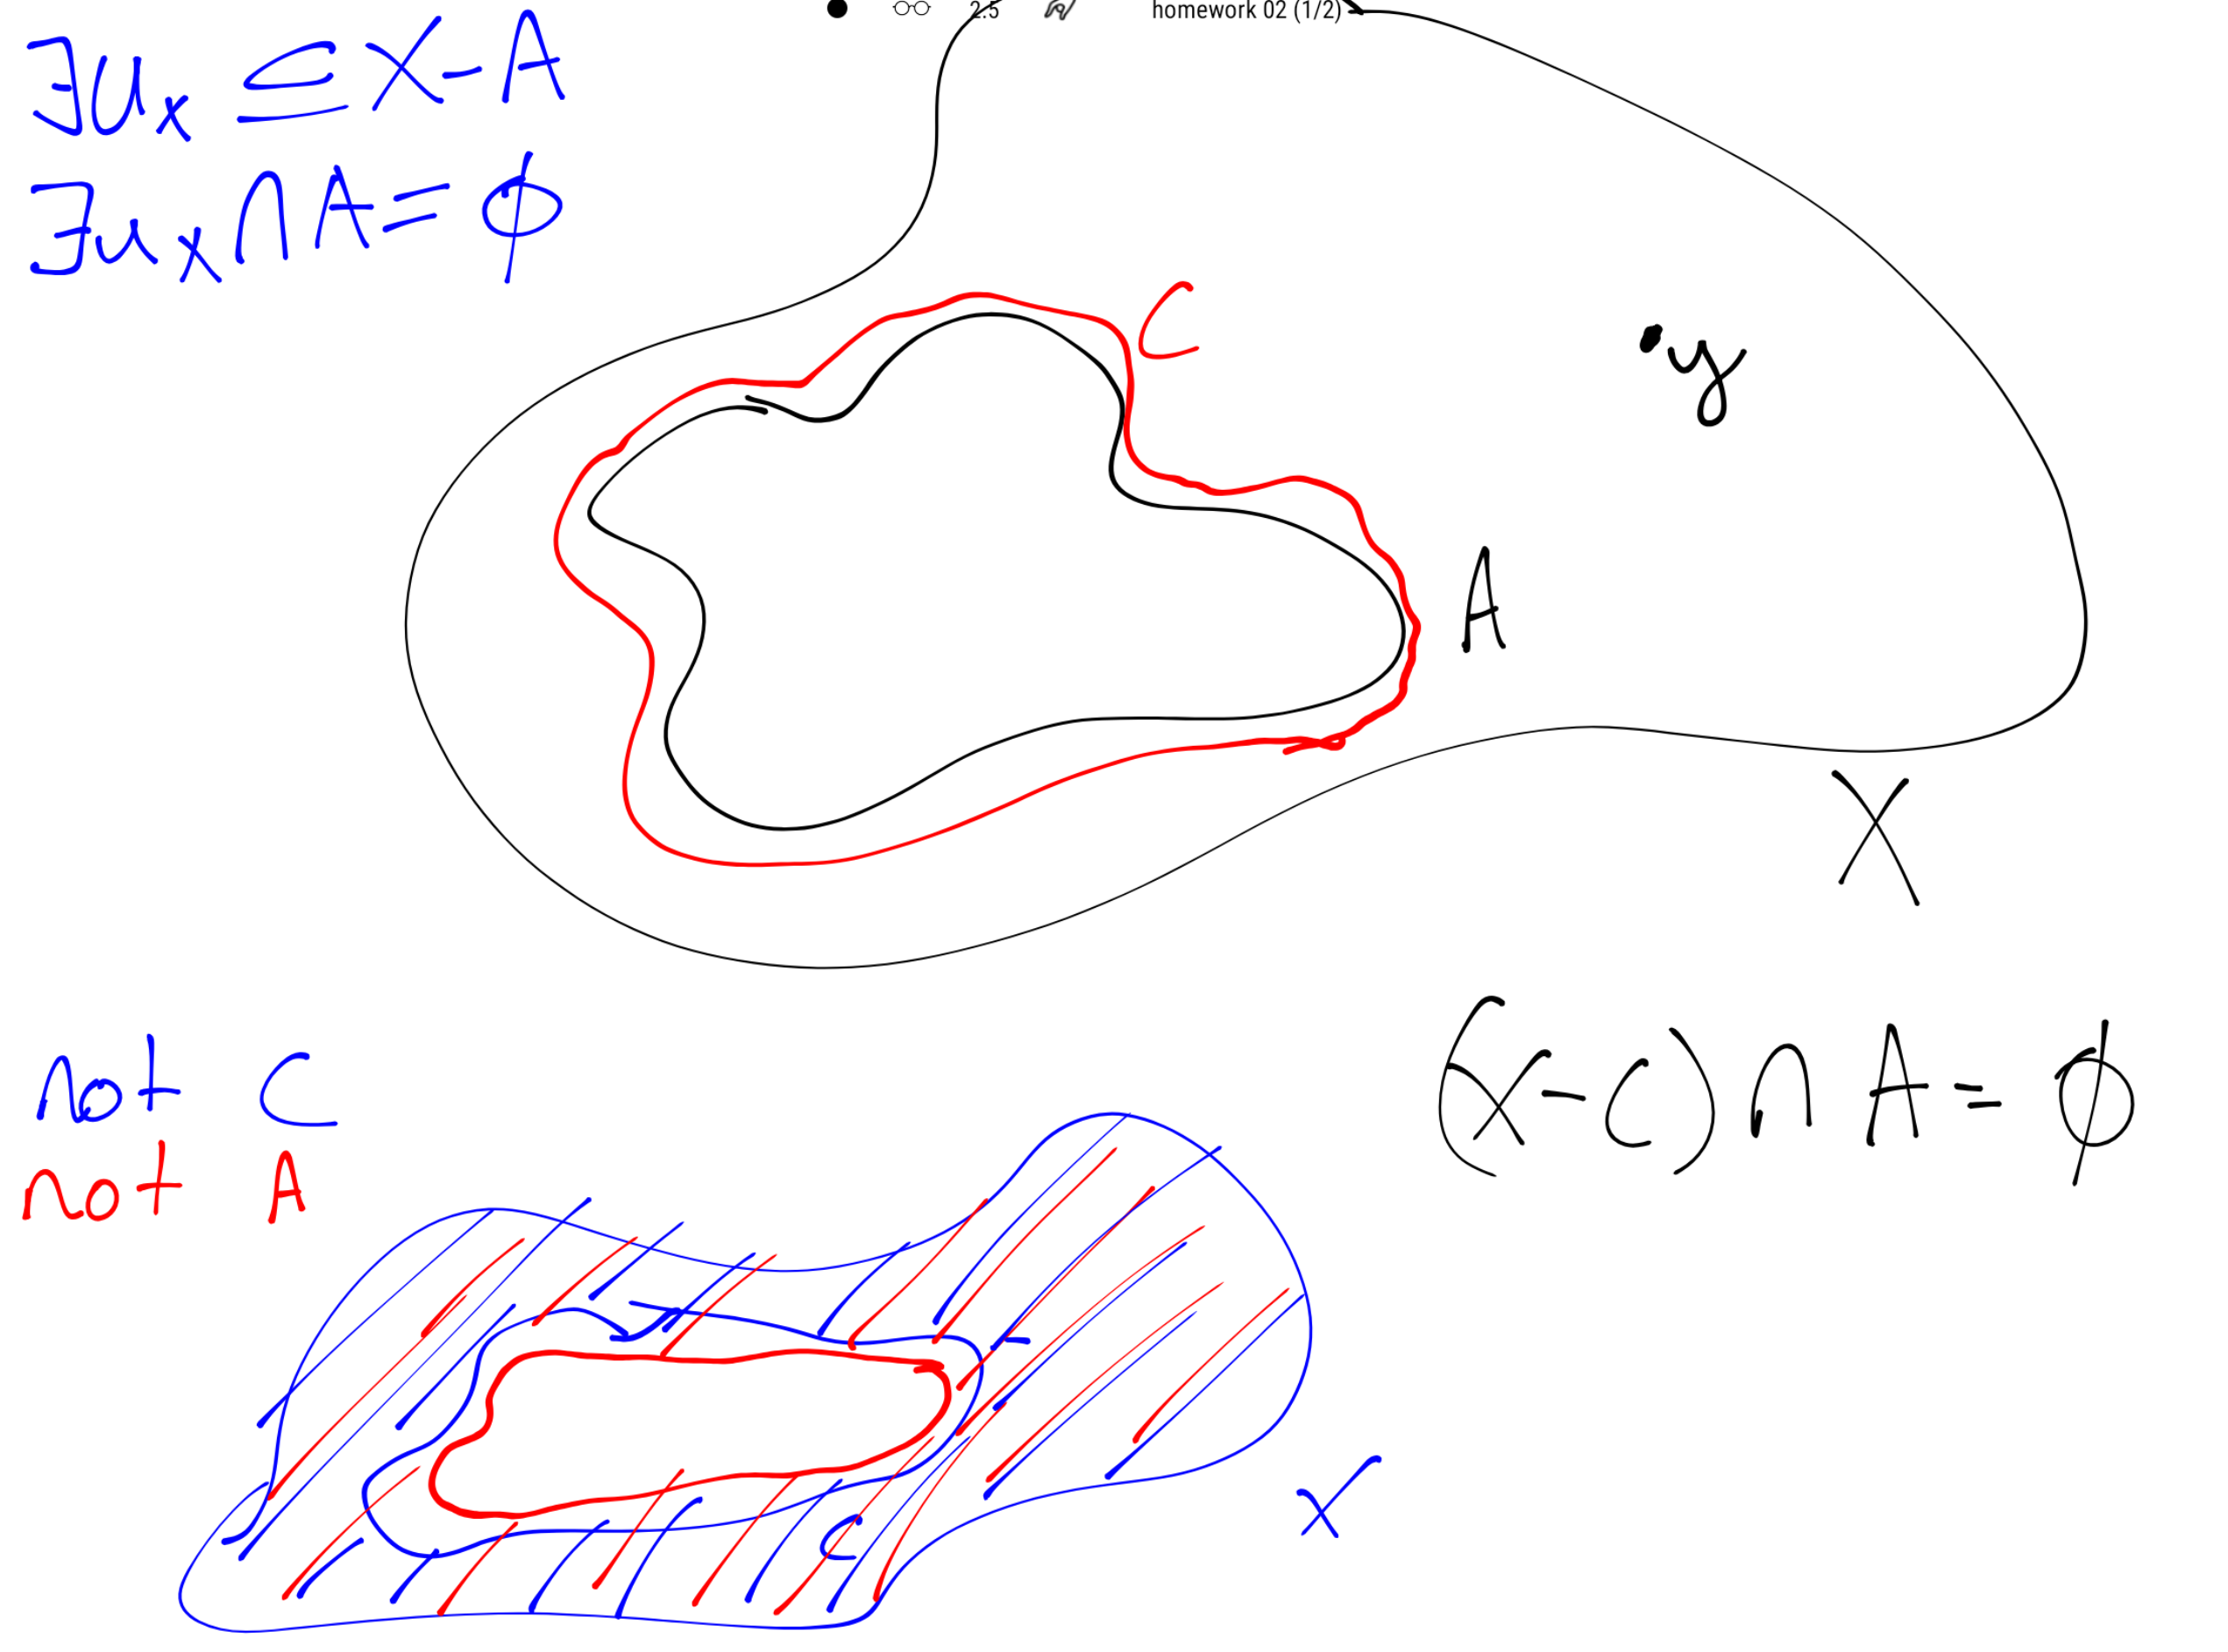
\includegraphics[height=10cm]{thm2.5.png}
\end{center}

If given a set $ X $ and $ A\subset X $. The complement of $ A $ is defined as $ X-A $. I don't really like this notation as it makes me think of subtraction, which isn't a wrong way to think of it, I just feel like this is more of the process of how we got the complement of $ A $ rather than actually being the complement.\\
\\
By instead thinking of not $ A $, I can think of the what $ A $ is not, rather than $ X-A $. This helps me have a better intuition of what is actually going on.


\newpage
\section{Failing \& Succeeding}

I feel like I am understanding the material much better as whole than last year when I took this course with Dr. George. I felt like I was completely lost for most of the semester. Each assignment I was faced with a struggle. While struggles are normally good and are a good indicator (cause?) growth. Struggling helps cement ideas and shows you where you're blind spots are. Without this struggle, much of mathematics will not stick pass the time line of an upcoming exam.\\
\\
Yet this was an unproductive struggle. I spent hours and hours staring at the paper, practically getting no where. Unproductive Struggle is incredibly frustrating, as it's a waste of time. I do not grow from the encounter and the work is still not completed.  I would scour the internet looking for help, but could not find much. I went to office hours multiple times a week and I would talk with friends about the problems. I specifically went on Sundays to the math tutoring center so that way Collin would be able to help guide me in the homework. (Colin was also taking the class at the same time as myself)\\
\\
Even with this ``Success" I still have a lot to do. I have done poorly on all my ``daily blood check up" quizzes. This is again interesting as I am close to understanding and feel like the answer is on the tip of my tongue. I feel like I am often times close to figuring out the proof, but I am missing some idea or exact wording that I can't double check during the quiz times to fully articulate the idea I want to use. \\
\\
I was particularly bad about working everyone day on topology. As I was freaking out over the reflection and homework due on Monday and Tuesday. I didn't spend much time learning the new material but instead focusing on "old" material that was on the homework. I also had another project due in one my grad classes and that took up Wednesday and Friday. \\
\\
On Thursday I competed in Mr. Heartthrob, a male beauty pageant and philanthropy event. In fact, I took home the title and won the competition. I had a blast and am very glad I participated. Mr. Heartthrob took up close to 8 hours of my week that I could have used to focus on school. I am still staying on top of it. I am just going to have some late nights here last week and this next week.

\newpage
\section{Notes to Myself}
I start out good on the weekends, spending several hours spaced out over the course of the day to work on the material. Yet throughout the rest of the week I do not work much on Topology. This is a poor way of doing it as it slowly makes me more and more behind. We are on week 4 or 5 now and I am now behind in my notes. I was a little behind the prior week and mostly on top of it the week prior to that. But little by little, I am now behind the material being taught in class.\\
\\
I need to work a little bit on Topology each and every day. Even spending 20 minutes before bed would be immensely beneficial to my understanding and doing well in this course. The biggest hurdle to doing so is being tired and busy with other obligations such as Work, Dance, and other classes. \\
\\
The hardest part for me is that I am taking 10 undergraduate credits, 6 graduate credits, working 18.5 hours a week, teaching dance lessons two nights a week for two hours each time, and hosting a social dance that takes up 4 hours every Friday.\\
\\
I have a hard time prioritizing all of it. I hate working all day, only to have to work all night. I am an incredibly social person and really just want to hang out and relax with others. I need this ``downtime" to help function.\\
\\
I need to get ahead this week. Turn in all your homeworks early and focus on school. If I can get ahead and will be able to stay on top of the ball. I am able to keep pace, I just want that pace to be a little further up ahead rather than right before it's due. \\
\\
\textbf{Remember}, just because a set is closed, it does not mean it is not open. A set can be both open and closed, clopen.\\
\\
Use your tablet more often for the homeworks and studying. The act of a blank canvas and writing down the ideas that come to mind will be greatly beneficial. It will help connect dots and provide more connected ideas with other concepts.\\
\\
I can embed the figures I draw into Notion. So, go crazy writing stuff down. It'll all be in the cloud indexable and organized. I can easily use this tool to relate and help my understanding as I continue the course.\\
\\
Go to office hours more. Even if its just for 5 or 10 minutes between classes, I believe this regularly visiting will help me out long term. Ideas and questions I hadn't thought of will be present. Connecting the dots and understand how it all fits together is the name of the game.\\
\\
If you're stuck, don't waste more than 10 minutes on the problem or idea. Afterwards, spend up to 10 minutes looking on the internet. If no progress is made then, write it down and ask Dr. Das for guidance.


\end{document} 